\chapter{Тестирование приложения} \label{chapt4}

По итогам разработки производятся тестовые испытания, позволяющие установить корректность функционирования разработанного программного комплекса и проверить соответствие функциональным требованиям. Логически, проект делится на серверную и клиентскую части. Основная задача серверной части - обработка сообщений и событий, приходящих от браузера, клиента. Самая сложная, нестабильная и слабопереносимая(между операционными системами) часть функциональности сервера состоит в автоматизации работы с программами RTKLIB. Именно этот модуль показал наименьшую стабильность при разработке и долговременном использовании. Дело в том, что ошибки при парсинге вывода этих программ, особенно управляемых интерактивной консолью, могут проявлять себя не сразу. Кроме того, данные модули являются критическими для приложения, ведь они предоставляются всю основную информацию, нужную для интерфейса. Таким образом, было решено создать модульные тесты для классов, управляющих работой RTKRCV, STR2STR и CONVBIN. Это позволило упростить разработку и дополнение этих классов новой функциональностью, без риска внести новые ошибки в код. Тестирование приложения можно разделить на две части:

\begin{enumerate}
  \item Тестирование модуля, отвечающего за работу с RTKLIB;
  \item Тестирование функциональности интерфейса;
\end{enumerate}

\section{Модульное тестирование классов, работающих с RTKLIB} \label{sect4_1}

Работа с модульными тестами будет рассмотрена на примере класса RtkController, автоматизирующего работу с RTKRCV. В качестве фрэймворка для юнит-тестирования был выбран стандартный для Python \textbf{unittest}.

Для создания тест-кейса при работе с unittest, требуется отдельный файл, описывающий сценарий нового теста. Тест в данном файле принимает форму класса, унаследованного от класса \textbf{unittest.TestCase}.

\lstinputlisting[
  label={listings:RtkController_test},
  caption={Класс RtkControllerTest},
  style={java}
]
{src/RtkController_test.py}

Методы данного класса представляют собой отдельные тесты. Также есть специальные методы, унаследованные от класса-родителя - \textbf{setUp} и \textbf{teadDown}. Эти методы следует переопределить, так как они вызываются при каждом из определенных пользователем тестов. В случае тестирования RtkController, setUp и tearDown переопределены для создания объекта класса RtkController и запуска RTKRCV до теста, а также остановки приложения после его выполнения. Такая структура класса позволит отделить запуск и остановку программы от функционального теста, проверяющего, например, получение корректного статуса, и таким образом получить более точные диагностические данные.

Перед каждым тестом, описанным ниже, вызывается RtkController.setUp(). Происходит проверка корректного запуска Rtkrcv с помощью метода \textbf{assertTrue}. Возврат значения False, а также любое брошенное исключение будет означать провал теста еще на этапе setUp.

\lstinputlisting[
  label={listings:RtkController_setUp},
  caption={Метод setUp класса RtkControllerTest},
  style={java}
]
{src/RtkController_setUp.py}

После успешного выполнения теста вызывается RtkController.tearDown(). После остановки RTKRCV, происходит проверка корректного завершения программы.

\lstinputlisting[
  label={listings:RtkController_tearDown},
  caption={Метод tearDown класса RtkControllerTest},
  style={java}
]
{src/RtkController_tearDown.py}

Тесты функциональности класса RtkController состоят в вызове других методов класса RtkController, например getStatus(). Этот метод сравнивает полученный объекта статуса с перечнем нужных параметров, которые выводит RTKRCV, чтобы проверить правильность парсинга вывода. Также, это происходит несколько раз подряд, для проверки надежности эмуляции консоли.

\lstinputlisting[
  label={listings:RtkController_testStatus},
  caption={Метод testStatus класса RtkControllerTest},
  style={java}
]
{src/RtkController_testStatus.py}

По такому же приниципу устроен тест метода getObs(). Однако, команда \textbf{obs} не возвращает информацию о спутниках при отключенной антенне, а значит достаточно получения пустого словаря и отсутствия брошенных исключений.

\lstinputlisting[
  label={listings:RtkController_testObs},
  caption={Метод testObs класса RtkControllerTest},
  style={java}
]
{src/RtkController_testObs.py}

\section{Функциональное тестирование интерфейса} \label{sect4_2}

Для данного прилоежния, тестирование интерфейса является тестированием на уровне приложения. Именно здесь проверяется корректность работы основых функций приложения - отображение статуса и настроек в режиме ровера, отображение настроек в режиме базы и отображение доступных логов спутниковых данных. В системе есть две возможности посмотреть логи приложения. В GNU/Linux, с помощью утилиты \textbf{journalctl} в составе \textbf{systemd} можно просматривать логи серверной части приложения. Для клиентской части приложения, в составе инструментов разработчика любого современного браузера, существует Javascript консоль. Контроль отсутствия ошибок в этих логах двух частей приложения и получение ожидаемых результатов работы гарантируют успешность тестов и корректность работы прилоежния. Для тестирования интерфейса были разработаны несколько методик, позволяющие проверить основные функции, выполняемые этим интерфейсом:

\begin{enumerate}
  \item Запуск приложения и состояние всех вкладок веб-страницы;
  \item Запуск режима ровера и получение корректного статуса, включая уровни спутников на графике;
  \item Изменение настроек RTKRCV и проверка, что эти изменения вступили в действие;
  \item Запуск режима базы и проверка получения поправок;
  \item Проверка возможности скачать лог в формате RINEX из списка логов;
\end{enumerate}

\subsection{Тестирование запуска и загрузки приложения} \label{subsect4_2_1}

\underline{Исходные данные.} Приложение не запущено.

\underline{Ожидаемый результат.} При запуске файла \textbf{server.py}, после сообщении о готовности сервера, на стандартном для HTTP 80 порту становится доступен разработанный веб-интерфейс. При открытии браузера и переходе на нужный IP адрес, открывается страница, состоящая из четырех вкладок: \textbf{Status}, \textbf{Config}, \textbf{Logs} и \textbf{Settings}. Состояние по умолчанию - незапущенный ровер. В логах, доступных при помощи \textbf{journalctl} отсутствуют ошибки.

\underline{Результат.} Совпал с ожидаемым. На группе рисунков 4.1 представлены вкладки описанной выше страницы при открытии в браузере смартфона.

\begin{figure}
  \label{img:latex}
  \begin{subfigure}{\linewidth}
    \center
    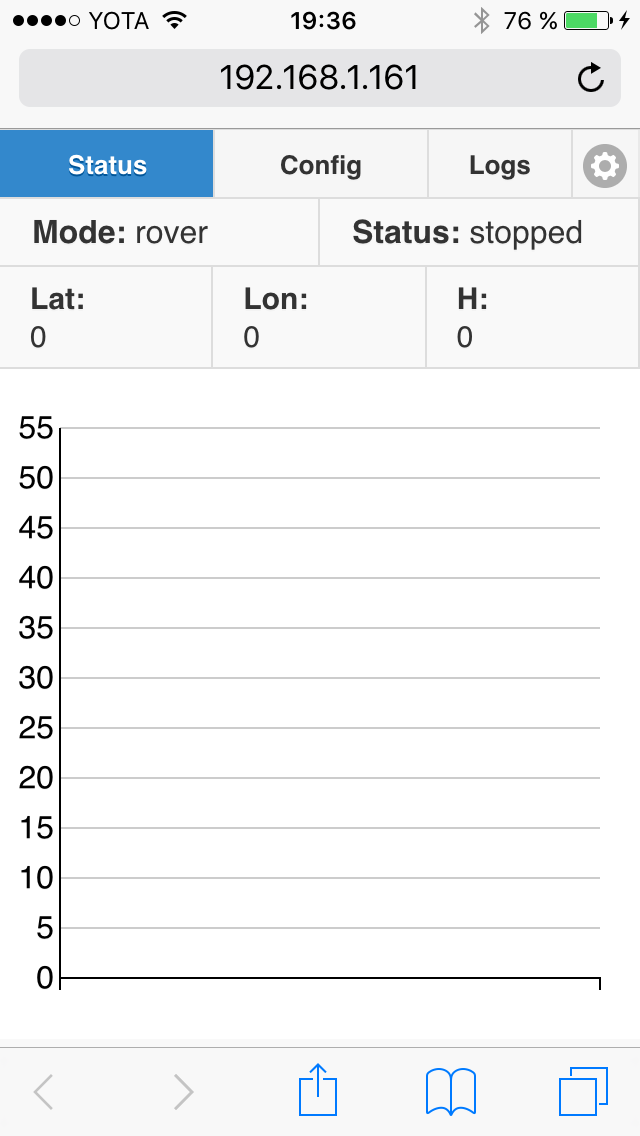
\includegraphics[width=.35\linewidth]{ui_testing_status_tab}
    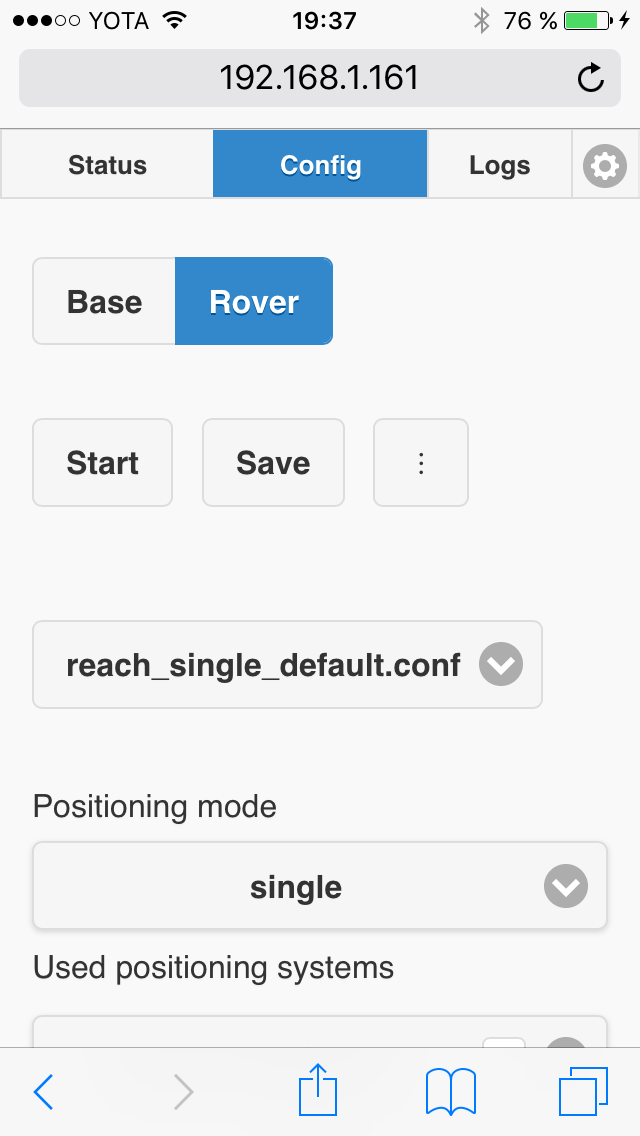
\includegraphics[width=.35\linewidth]{ui_testing_config_tab}
    \caption{Status и Config}
  \end{subfigure}\par\medskip
  \begin{subfigure}{\linewidth}
    \center
    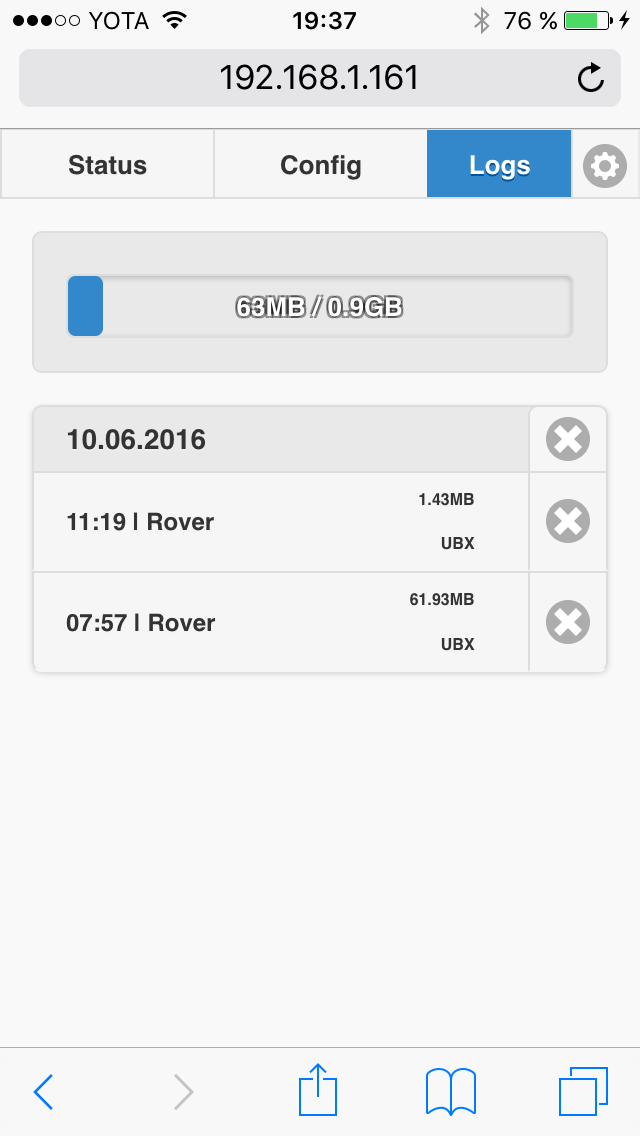
\includegraphics[width=.35\linewidth]{ui_testing_logs_tab}
    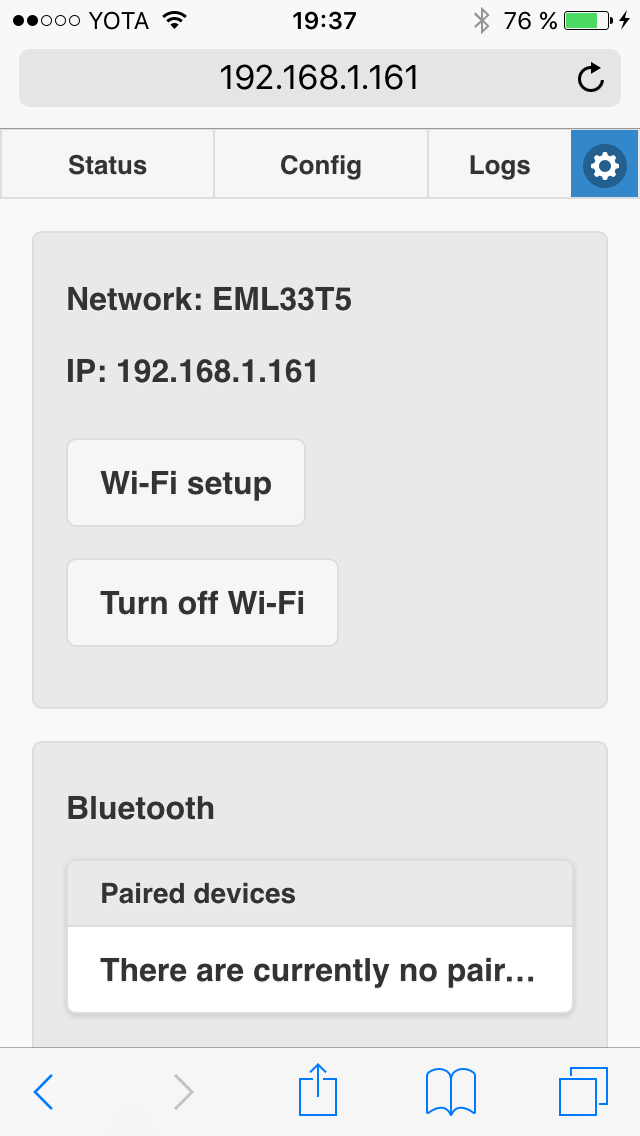
\includegraphics[width=.35\linewidth]{ui_testing_settings_tab}
    \caption{Logs и Settings}
  \end{subfigure}\par\medskip
  \caption{Вкладки приложения в браузере смартфона}
\end{figure}

\subsection{Тестирование работы режима ровера} \label{subsect4_2_1}

















